\documentclass[handout,instructornotes]{ximera}
%handout:  for handout version with no solutions or instructor notes
%handout,instructornotes:  for instructor version with just problems and notes, no solutions
%noinstructornotes:  shows only problem and solutions

%% handout
%% space
%% newpage
%% numbers
%% nooutcomes

%I added the commands here so that I would't have to keep looking them up
%\newcommand{\RR}{\mathbb R}
%\renewcommand{\d}{\,d}
%\newcommand{\dd}[2][]{\frac{d #1}{d #2}}
%\renewcommand{\l}{\ell}
%\newcommand{\ddx}{\frac{d}{dx}}
%\everymath{\displaystyle}
%\newcommand{\dfn}{\textbf}
%\newcommand{\eval}[1]{\bigg[ #1 \bigg]}

%\begin{image}
%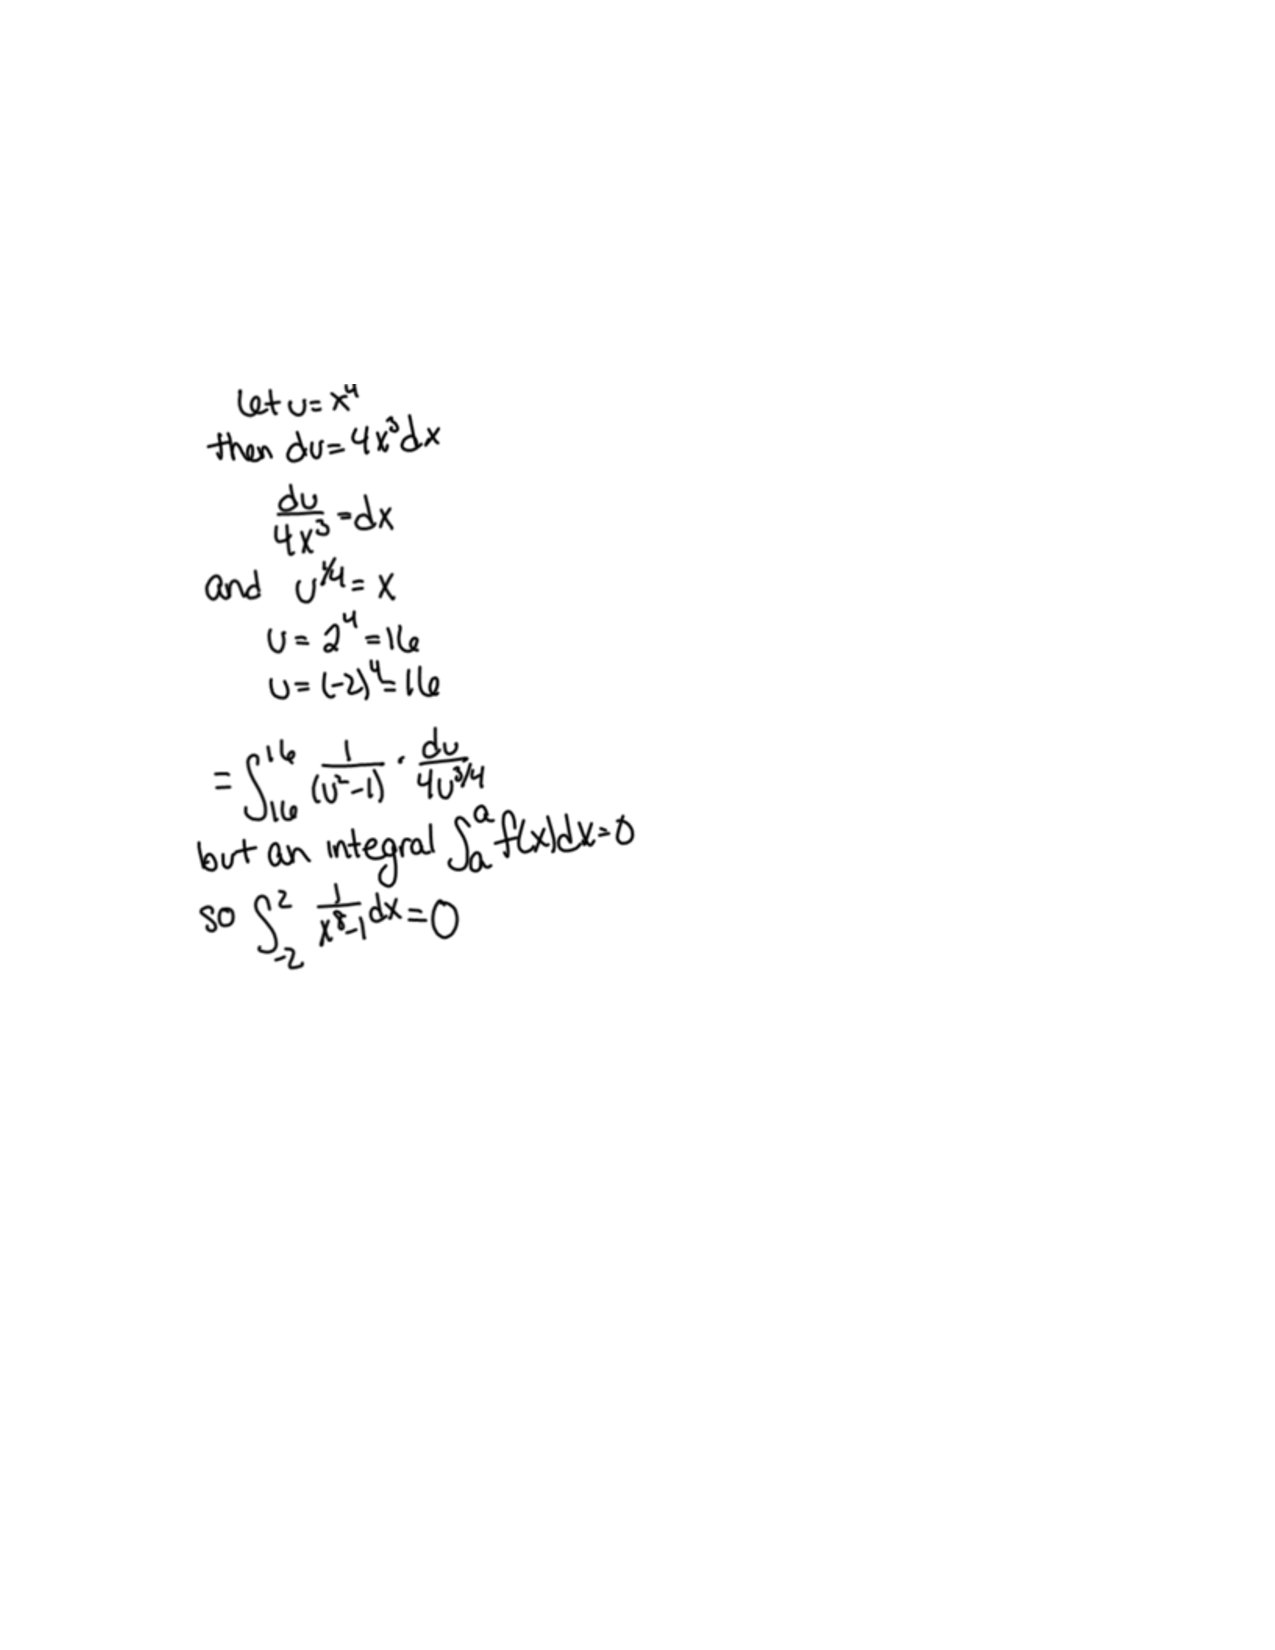
\includegraphics[trim= 170 420 250 180]{Figure1.pdf}
%\end{image}

%add a ``.'' below when used in a specific directory.
\newcommand{\RR}{\mathbb R}
\renewcommand{\d}{\,d}
\newcommand{\dd}[2][]{\frac{d #1}{d #2}}
\renewcommand{\l}{\ell}
\newcommand{\ddx}{\frac{d}{dx}}
\newcommand{\dfn}{\textbf}
\newcommand{\eval}[1]{\bigg[ #1 \bigg]}

\usepackage{multicol}

\renewenvironment{freeResponse}{
\ifhandout\setbox0\vbox\bgroup\else
\begin{trivlist}\item[\hskip \labelsep\bfseries Solution:\hspace{2ex}]
\fi}
{\ifhandout\egroup\else
\end{trivlist}
\fi} %% we can turn off input when making a master document

\title{Recitation \#19: Approximating functions with polynomials - Instructor Notes}  

\begin{document}
\begin{abstract}		\end{abstract}
\maketitle



\section{Warm up:}
For each of the following, write the given polynomial in summation notation starting with $k=0$.
	\begin{enumerate}
	
	\item  $\frac{3x}{2} - \frac{5x^2}{3} + \frac{7x^3}{4} - \frac{9x^4}{5} + \frac{11x^5}{6}$
	
	\item  $\frac{1}{2}x + \frac{1 \cdot 5}{4 \cdot 2!}x^3 + \frac{1 \cdot 5 \cdot 9}{8 \cdot 3!}x^5 - \frac{1 \cdot 5 \cdot 9 \cdot 13}{16 \cdot 4!}x^7$
	
	\item  $(x-1)^3 - \frac{(x-1)^4}{2!} + \frac{(x-1)^5}{4!} - \frac{(x-1)^6}{6!} $
	
	\end{enumerate}
	
	\begin{freeResponse}
	\begin{enumerate}
	
	\item  $\sum_{k=0}^4 (-1)^k (2k+3) \frac{x^{k+1}}{k+2}$.  
	
	\item  $\sum_{k=0}^3 \frac{1 \cdot 5 \cdot \hdots \cdot (4k+1)}{2^{k+1} (k+1)!} x^{2k+1}.$
	
	\item  $\sum_{k=0}^3 \frac{(-1)^k}{(2k)!} (x-1)^{k+3}$.  
	
	\end{enumerate}
	\end{freeResponse}
	
\begin{instructorNotes}
Maybe give one problem per group.  
Allow $4$ minutes for group work and $6$ minutes for discussion.  
Make sure to note that we can ``factor out'' terms dealing only with $x$, but not with $k$ (or $n$).  
Also, you might want to discuss starting with $k$ equaling another number other than $0$.
\end{instructorNotes}







\section{Group work:}



%problem 1
\begin{problem}
Assuming that the function $f(x)$ is infinitely differentiable, and given that
	\[
	f(x) = f(a) + \frac{f'(a)}{1!}(x-a)^1 + \frac{f''(a)}{2!}(x-a)^2 + \frac{f'''(a)}{3!}(x-a)^3 + c_4 (x-a)^4 + \frac{f^{(5)}(a)}{5!}(x-a)^5
	\]
show that the coefficient $c_4$ of the $(x-a)^4$ term in the Taylor polynomial is $\frac{f^{(4)}(a)}{4!}$.  
	\begin{freeResponse}
	Notice that we have the following:
		\begin{align*}
		&f'(x) =  f'(a) + f''(a)(x-a) + \frac{f^{(3)}(a)}{2} (x-a)^2 + 4 c_4 (x-a)^3 + \frac{f^{(5)}(a)}{4!}(x-a)^4  \\
		&f''(x) =  f''(a) + f^{(3)}(a) (x-a) + 4 \cdot 3 c_4 (x-a)^2 + \frac{f^{(5)}(a)}{3!}(x-a)^3  \\
		&f^{(3)}(x) =  f^{(3)}(a) + 4 \cdot 3 \cdot 2 c_4 (x-a)  + \frac{f^{(5)}(a)}{2}(x-a)^2 \\
		&f^{(4)}(x) =   4! \cdot c_4 + f^{(5)}(a)(x-a)  \\
		&f^{(4)}(a) = 4! \cdot c_4 + 0  \\
		&\Longrightarrow \qquad \boxed{c_4 = \frac{f^{(4)}(a)}{4!}}.
		\end{align*}
	\end{freeResponse}
	
\end{problem}

\begin{instructorNotes}
The lecture justifies the coefficients of $p_3(x)$.  
This problem should be done as a whole class discussion, perhaps for about $5$ minutes.  
\end{instructorNotes}







%problem 2
\begin{problem}
Let $f(x) = \sin(2x)$.  
Find $p_3(x)$ about the point $a = \frac{\pi}{8}$.  
	\begin{freeResponse}
	First, note that around $a$
		\[
		p_3(x) = f(a) + f'(a)(x-a) + \frac{f''(a)}{2}(x-a)^2 + \frac{f^{(3)}(a)}{3!}(x-a)^3.
		\]
	So we compute
		\begin{align*}
		&f'(x) = 2 \cos(2x) 	\quad	\Longrightarrow	\quad	f' \left( \frac{\pi}{8} \right) = \sqrt{2}  \\
		&f''(x) = -4\sin(2x) 	\quad	\Longrightarrow	\quad	f'' \left( \frac{\pi}{8} \right) = - 2 \sqrt{2}  \\
		&f^{(3)}(x) = -8\cos(2x)	\quad	\Longrightarrow	\quad	f^{(3)} \left( \frac{\pi}{8} \right) = -4\sqrt{2}.
		\end{align*}
	Therefore
		\[
		\boxed{p_3(x) = \frac{\sqrt{2}}{2} + \sqrt{2} \left( x - \frac{\pi}{8} \right) - \sqrt{2} \left( x - \frac{\pi}{8} \right)^2 - \frac{2\sqrt{2}}{3} \left( x - \frac{\pi}{8} \right)^3}.
		\]
	\end{freeResponse}
		
\end{problem}

\begin{instructorNotes}
Students often have difficulty ``putting the pieces together'', particularly when $a \neq 0$.  
Watch for students not putting the polynomial as powers of $\left(x - \frac{\pi}{8} \right)$.  
They often will just use powers of $x$.  
They also will often not plug in $\frac{\pi}{8}$ into the derivative (leaving the derivative in terms of $x$).  
Another common error is forgetting the $k!$.  
\end{instructorNotes}







%problem 3
\begin{problem}
Let $f(x) = xe^{-x}$ on the interval $[-2,8]$.  
	\begin{enumerate}
	
	\item  Write the Taylor polynomial $p_4(x)$ around $a=3$.
		\begin{align*}
		\text{Fun facts: } f'(x) &= -e^{-x}(x-1)  \\
		f''(x) &= e^{-x} (x-2) \\
		f^{(3)}(x) &= -e^{-x} (x-3) \\
		f^{(4)}(x) &= e^{-x} (x-4) 
		\end{align*}
	
	\item  Write $p_4(x)$ about $a=3$ in summation notation.  
	Also, write the remainder term $R_4(x)$.  
	
	\item  Calculate $p_4(4.5)$ and, using $R_4(4.5)$, estimate how close $p_4(4.5)$ is to $f(4.5)$.  
	Do the same for $p_4(1.5)$.  
	
	\item  Use the remainder term $R_4(x)$ to estimate the maximum error for $p_4(x)$ on $[-2,8]$.
	
	\item  How large must $n$ be to assure that the $n^{th}$ degree Taylor polynomial for $f(x) = xe^{-x}$ about $a=3$ approximates $2e^{-2}$ within $10^{-5}$?
	
	\end{enumerate}
	
	\begin{freeResponse}
	\begin{enumerate}
	
	\item  
		\begin{align*}
		p_4(x) &= f(a) + f'(a)(x-a) + \frac{f''(a)}{2!}(x-a)^2 + \frac{f^{(3)}}{3!}(x-a)^3 + \frac{f^{(4)}}{4!}(x-a)^4  \\
		&= 3e^{-3} -2e^{-3}(x-3) + \frac{e^{-3}}{2}(x-3)^2 - \frac{e^{-3}}{4!}(x-3)^4.
		\end{align*}
	
	\item  
		\[
		p_4(x) = \sum_{k=0}^4 \frac{(-1)^k e^{-3} (3-k)}{k!}(x-3)^k.
		\]
		\[
		R_4(x) = f(x)-p_4(x) = \frac{f^{(5)}(c)}{5!}(x-3)^5 = \frac{-e^{-c} (c-5)}{5!}(x-3)^5
		\]
	for some $c$ between $x$ and $3$.
	
	\item  
	
	\item  
	
	\item  
	
	\end{enumerate}
	\end{freeResponse}

\end{problem}

\begin{instructorNotes}
This is the longest of the problems.  
Part (a) is like the preceeding problem, where they need to remember to plug $3$ into the derivatives.  
For part (b), they also need to recognize that $R_4(x)$ deals with $f^{(5)}(x)$ and not $f^{(4)}(x)$.  
Writing $R_4(x) = \frac{f^{(5)}(c)}{5!} (x-3)^5$ for some $c \in [-2,8]$ will be sufficient at this stage (they will bound $f^{(5)}(c)$ in parts (c) and (d)).  

In part (c), the main issue is to bound $|f^{(5)}(x)| = |-e^{-5}(x-5)|$ on $[3,4.5]$ and $[1.5,3]$, and on $[2,8]$ for part (d).  
This is a problem of finding the absolute max (and min) of a function on a closed interval.  
Students then need to find critical value(s) by finding when $f^{(6)}(x) = 0$ (or undefined) as well as consider endpoints $f^{(6)}(x) = e^{-x}(x-6)$, with critical $x=6$.  
The last hurdle is to recognize we want to find the max of $|f^{(5)}(x)|$.  
This maximum occurs at $x=3, x=1.5$, and $x=-2$ respectively.
\end{instructorNotes}
















	
	
	
	
	
	
	
	
	

	










								
				
				
	














\end{document} 


















